\documentclass[12pt]{unlsilabsop}
\title{Module assembly: Encapsulation of wirebonds}
\date{August 6, 2015}
\author{Frank Meier Aeschbacher, José Andres Monroy}
\approved{Frank Meier Aeschbacher}
\sopid{105}
\sopversion{v1}
\sopabstract{Describes the procedures to encapsulate wirebonds of modules using the robotic gantry. The procedure takes place in the clean room.}

\usepackage{graphicx}

\begin{document}

\maketitle

%------------------------------------------------------------------
\section{Scope}
This is a regular part in the manufacturing process of pixel modules at UNL.

%------------------------------------------------------------------
\section{Purpose}
Wirebonds should receive protection by applying an encapsulant. This is the final manufaturing step.

%------------------------------------------------------------------
%>\section{Definitions}

%------------------------------------------------------------------
%\section{Responsibilities}

%------------------------------------------------------------------
\section{Equipment}
\begin{figure}[h]
    \begin{center}
        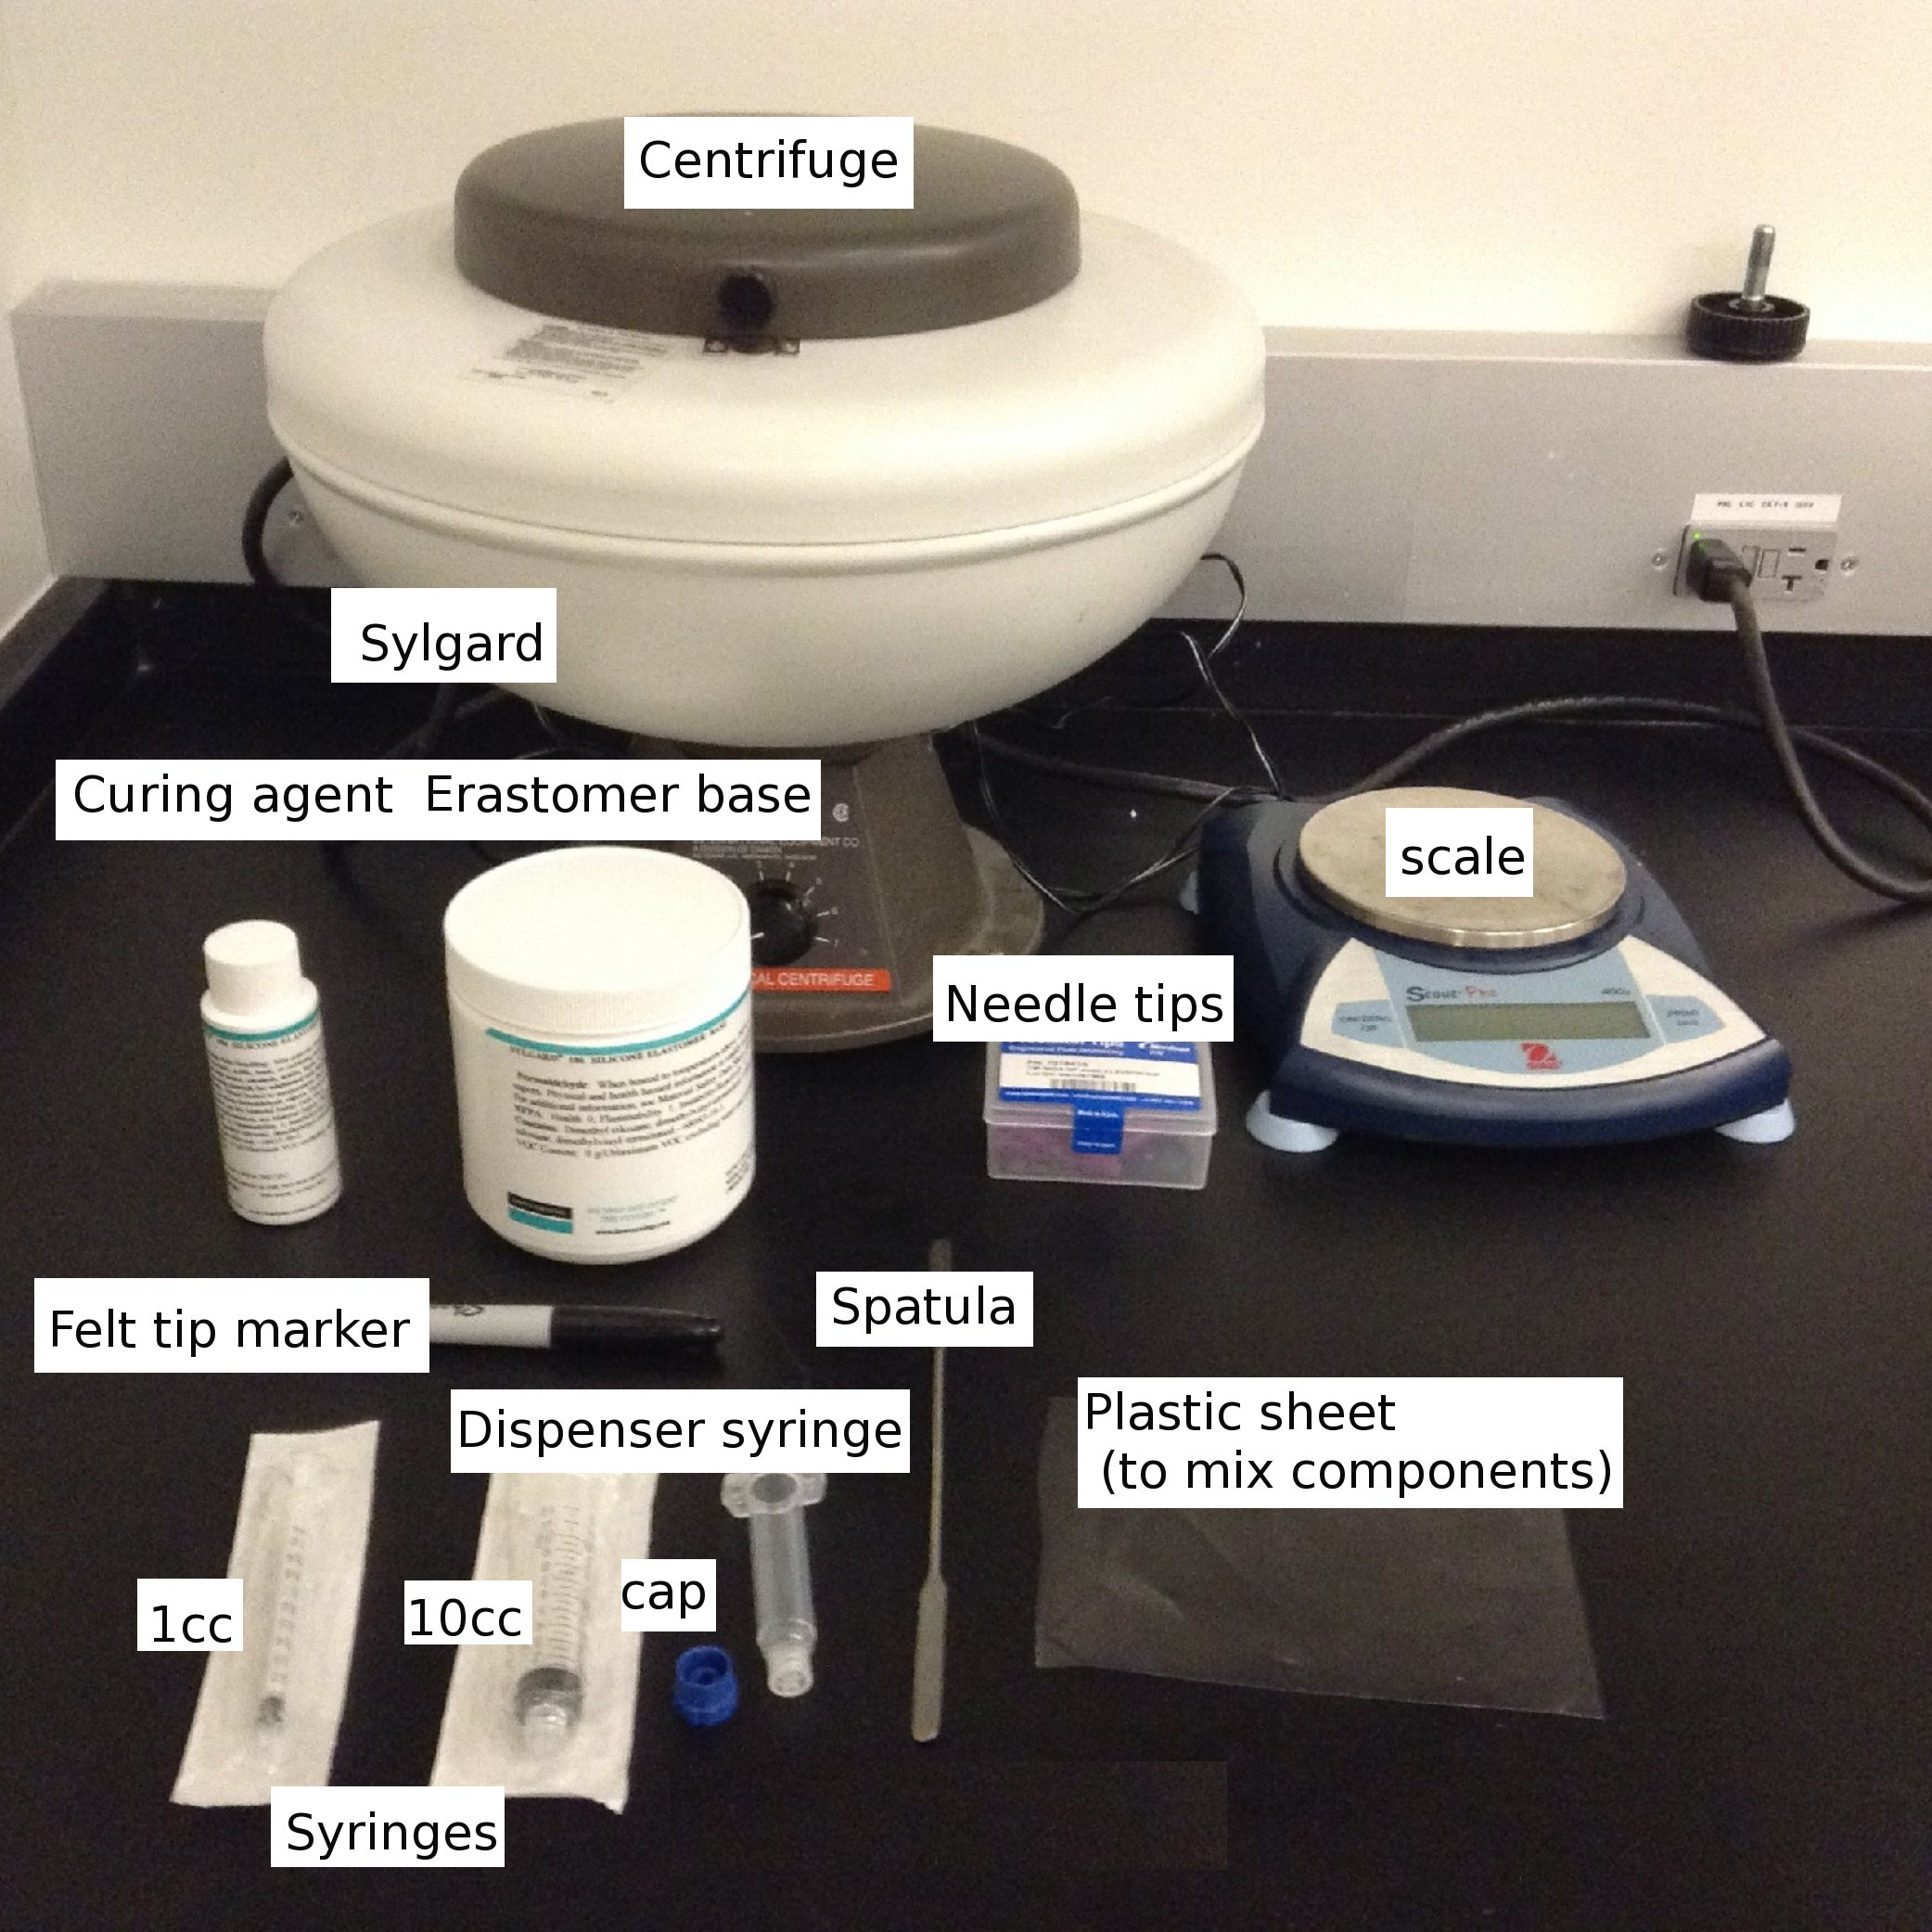
\includegraphics[scale= 0.3]{img/potting_materials.jpg}
        \caption{Material to prepare Sylgard}
        \label{fig:pottingmaterial}
    \end{center}
\end{figure}

\begin{figure}[h]
  \begin{center}
    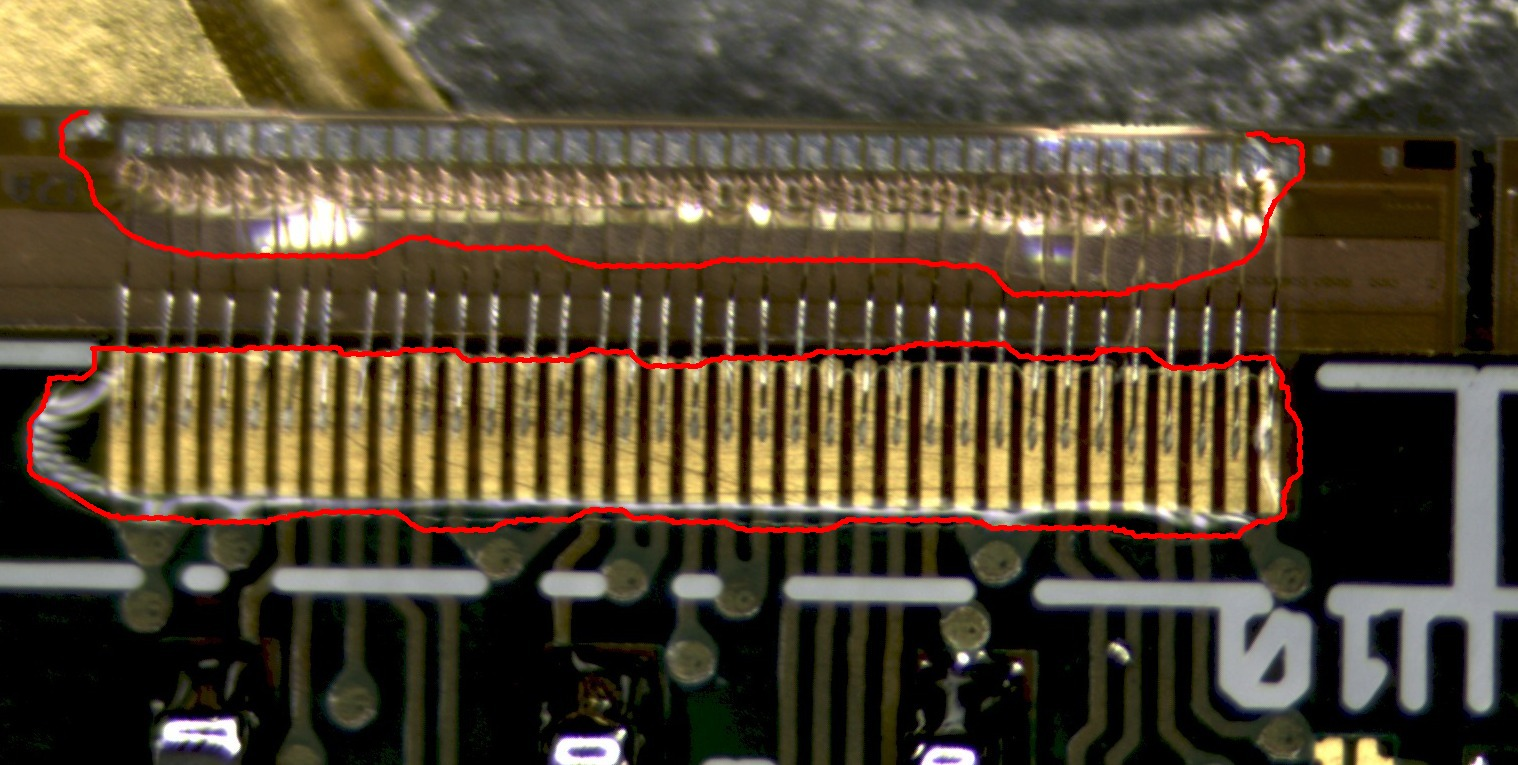
\includegraphics[width=\textwidth]{img/potting_reference.jpg}
    \caption{ROC-HDI encapsulation sample for comparison, all the bond foots and pads are fully covered as needed. The boundaries of the encapsulant enhanced with red lines for better visibility.}
    \label{fig:potting_reference}
  \end{center}
\end{figure}

\begin{figure}[h]
    \begin{center}
        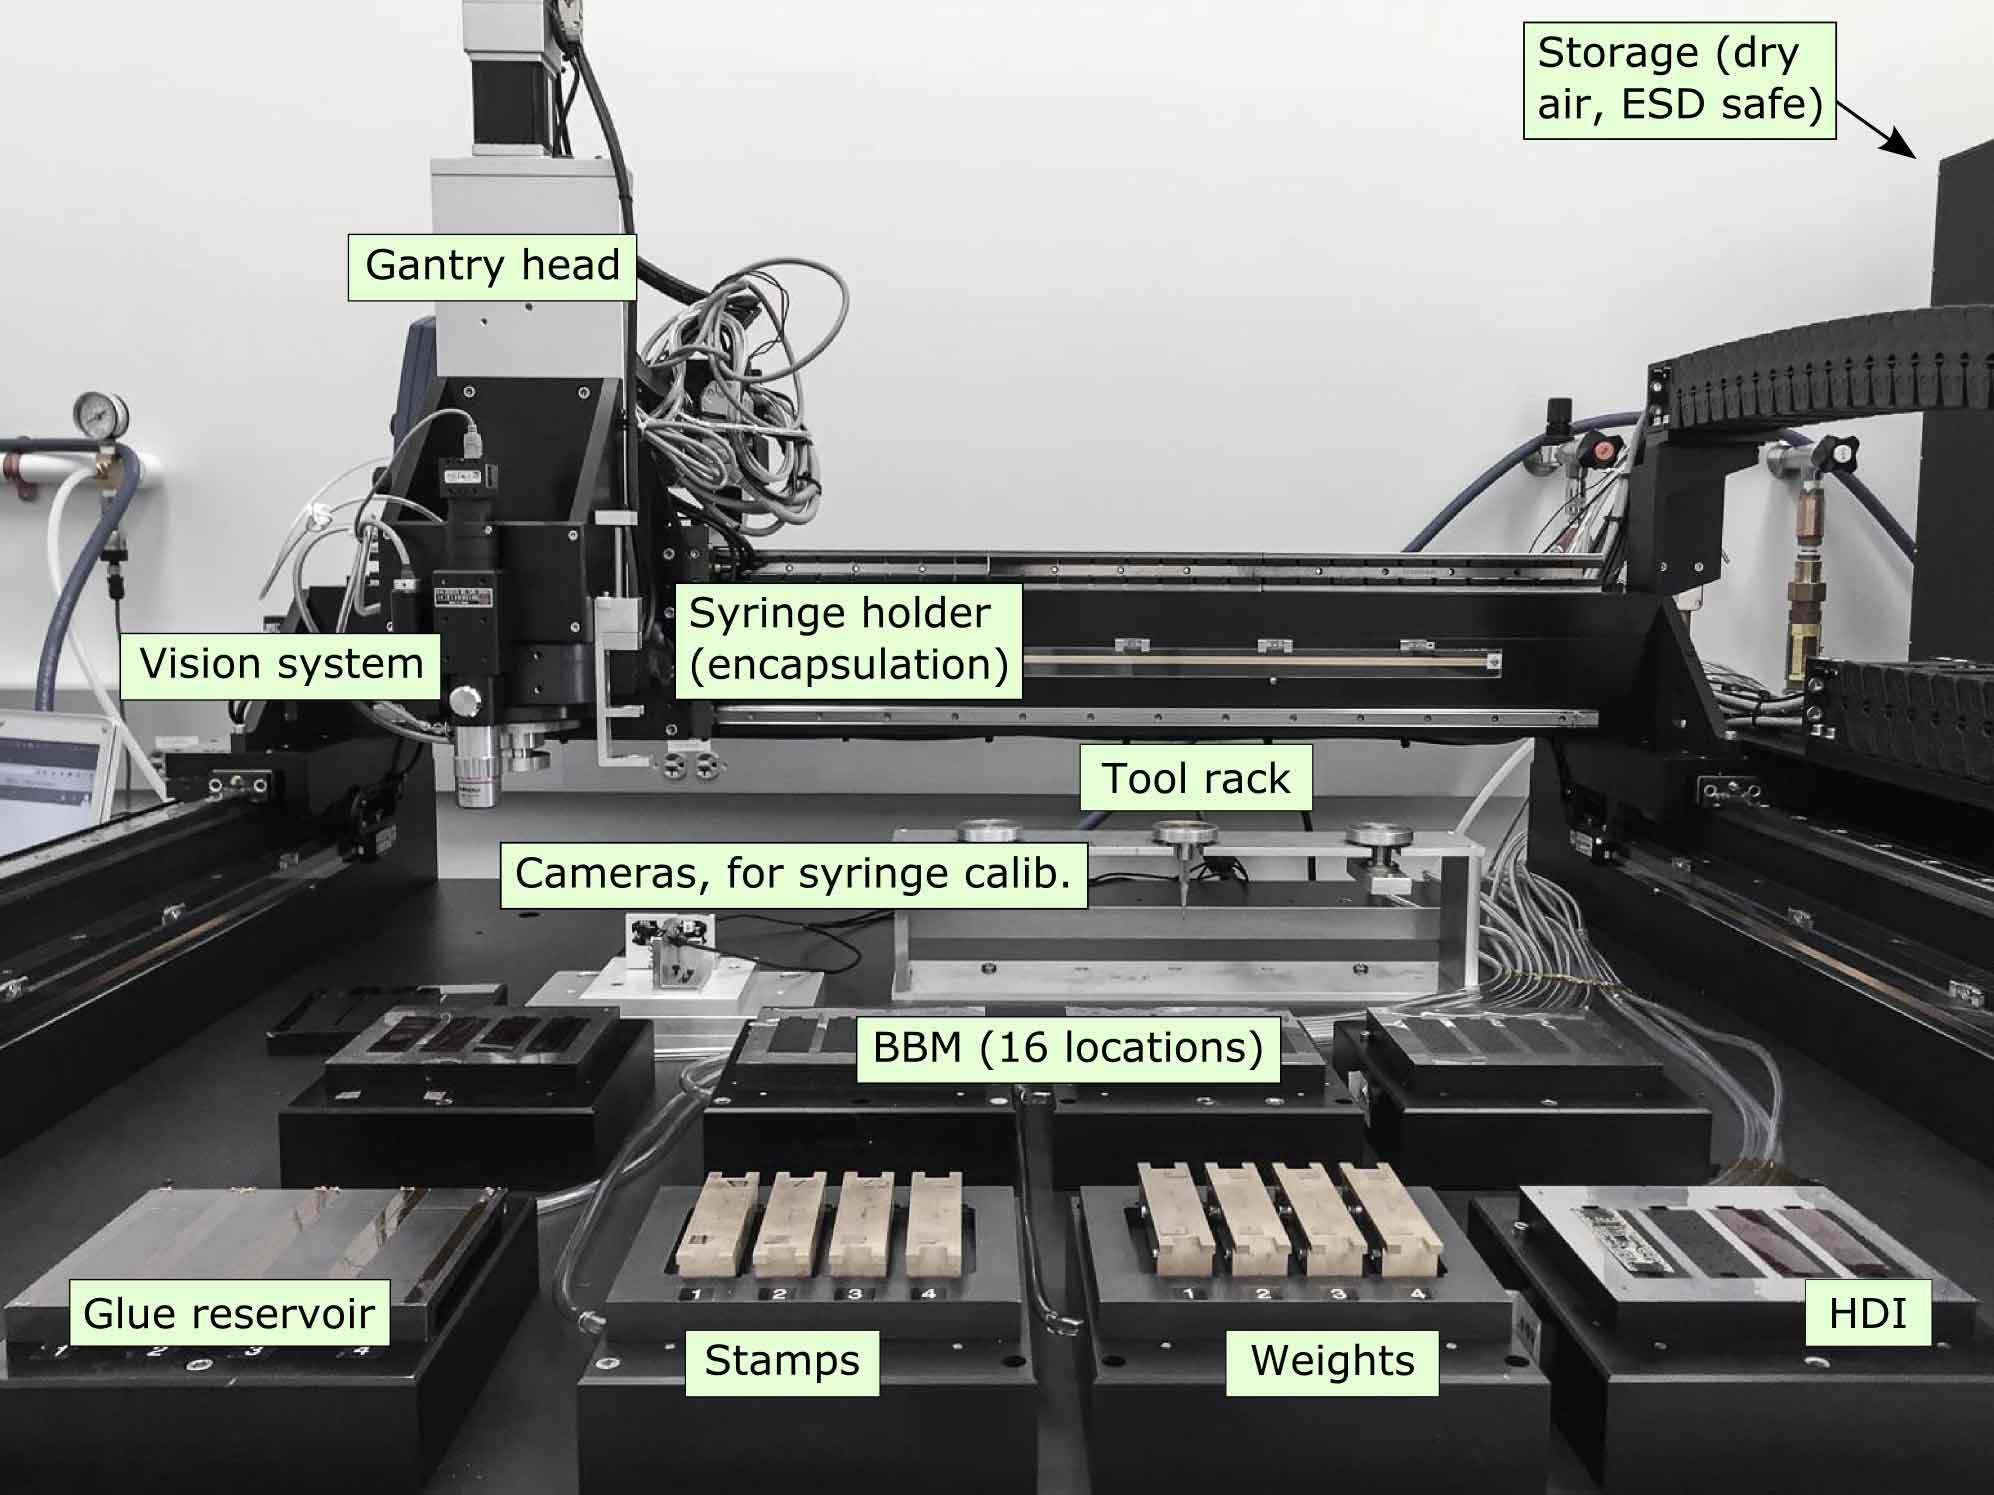
\includegraphics[width=\textwidth]{img/gantryFull16labeled.jpg}
        \caption{Gantry setup. The gantry is used for glueing too (SOP-103). For encapsulation, the relevant parts are the gantry head, the vision system, the syringe holder, the cameras for syringe calibration and the BBM chucks. Note: arrangement may vary as long as it matches the setup in the software.}
        \label{fig:gantryFullLabeled}
    \end{center}
\end{figure}

\begin{itemize}
    \item Gantry
    \item Nordson ESD Ultumus I dispenser
    \item Chucks equipped with carrier chucks for modules
    \item Encapsulant: Sylguard 186 two-component encapsulant. Consists of erastomer base and elastomer curing agent.
    \item Test tube to mix encapsulant
    \item Electronic scale.
    \item Spatula
    \item Disposable syringes for measuring volumes: 1\,cc size for curing agent and 10\,cc size for base
    \item Disposable syringe for dispenser, 5\,cc size, Nordson ESD, part no.~7012094
    \item Dispenser needle, color code: lavender, Nordson ESD part no. 7018433
    \item Disposable end cap for syringe, 5\,cc size, Nordson ESD, part no.~7012192
    \item Centrifuge
    \item Polyimide sheets, to cover chuck positions if not running a full batch of 4 modules
    \item Felt tip marker, to write batch number on chuck
    \item Curing oven
    \item Empty module carriers, amount matching number of modules to be encapsulated
    \item Allen key (TODO: add size)
    \item Binder clip, 15\,mm wide, inside insulated with Kapton tape
\end{itemize}

%------------------------------------------------------------------
\section{Procedure}

The procedure below is good for encapsulation of a larger number of modules than just the 4 of one chuck.
\begin{enumerate}
    \item Handle modules only with proper protection: ESD wristband, gloves, face mask.
    \item Perform a readiness check of the gantry:
    \begin{enumerate}
	\item Test presence of vaccum on the gauge, record the pressure.
	\item Test presence of compressed air by engaging the dispenser
        \item Turn on the Npaq controller and the power supply (located in the rack below the Npaq)
        \item Open LabView control software ``potting\_dev\_version(main)'' located at $$ \sim\backslash MyDocuments\backslash andres\backslash routine\backslash development\backslash potting \backslash potting\_dev\_version(main)$$
        \item Start the A3200 motion composer sofware (taskbar) and connect the controller by pressing the ``connect'' button.
       \item Pick modules from storage and identify them. Check that the parts satisfy the quality criteria by retrieving their information in the database. \label{enum:startenacpulation}
    \item Record the UNL id (\texttt{Nxxxyy}) for each module. Write down the number on the edge of the chuck for further identification.
    \end{enumerate}
  \item Run the LabVIEW control software. Supervise progress and stop in need, especially when modules are at risk. Some pop-up windows will appears asking for information:
    \begin{enumerate}
    \item is the vacuum active?
    \item distribution to be used (spots in use).  
    \item modules identification.  
    \end{enumerate}
  \item Run pattern recognition step by pressing the ``1.~Find potting reference positions'' button. (The camera will go through the HDI's potting positions and then through the modules potting positions)
    \begin{enumerate}
    \item Select the configuration to be used: test$\to$ testing purpose; HDIV3 + module $\to$ module encapsulation (wait 30 seconds while the program is loading some data). 
    \item First part is the fiducial recognition: for every single fiducial, check if location found is sound. After go through the 4 fiducials a pop-up window will ask if any of the found positions needs to be corrected. If the fiducial is not found, the manual mode becomes active, use the joystick to define the fiducial position. The manual mode is accesible anytime by pressing the ``switch to manual mode'' button.   
    \item Second part is the potting reference positions definition: Adjust the positions using the joystick and define them position by pressing the ``capture position'' button. Pay special attention to the focus (z coordinate); recall, there are 82 positions/module to be defined. 
    \item Write comments if any and press the ``send comments'' button to finish the step .
    \end{enumerate}
  \item Prepare encapsulant in lab outside the cleanroom:\label{enum:prepencapsulant}
    \begin{enumerate}
        \item Check expiration date of both ingredients. Replace if expired.
	\item Record batch number and expiration date of encapsulant.
        \item put a piece of paper on the electronic scale an adjust the zero.
	\item Take $\approx$ 0.3\,cc of curing agent using the 1\,cc syringe and deposit 0.3\,g on the paper in the scale. Adjust the zero again 
        \item Take $\approx$ 3.0\,cc of base elastomer using the 10\,cc sysringe and deposit 3.48\,g on the paper in the scale. Take the paper from the scale and mix the ingredients
        \item Transfer the mixture to the dispenser syringe (dont forget to use the end cap).  
	\item Fill another test tube with water
	\item Place both tubes in centrifuge at opposite location to balance rotor.
	\item Centrifuge for 2\,min. Repeat until encapsulant shows no bubbles anymore.
	\item Transfer syringe into cleanroom
    \end{enumerate}
    \item Attach tube to syringe and insert syringe into holder at gantry head (end cap has to be removed).
    \item Install the needle.
    \item Run the Encapsulation by pressing the ``2.~Encapsulation'' button. a pop-up window will ask you for install the syringe into the holder which should be already done.
    \item proceed to determine (calibrate) the position of the needle tip. A pop-up window will appears showing the image from the camera 2 in the webcam setup. Use the joystick to move the gantry until the needle tip is in the center of the screen (the center of the needle tip coincides with the red cross in the screen), then switch to camera 3 and repeat the process, once the needle tip is in the center of both images (from cameras 2 and 3) press the button ``calibrate''.
    \item Purge the syringe by pressing the ``Purge'' button (as requested by the pop-up window).
    \item Start the encapsulation by pressing the button ``start potting''. A control will appears asking for uncheck the irregular wirebonds or the sylgard traces that must be skipped.     
    \item At the end of the full cycle, check visually if all wirebond foots are covered as needed (see fig. \ref{fig:potting_reference} for reference); record observations in the comments box.
    \item Write comments and press the ``send comments'' button to finish the step. 
    \item Press the ``Finish'' button, a pop-up window will ask for final-additional comments.
    \item press the ``create report and finish'' button to create the report. provide the required information and press send.
    \item To correct for any missing encapsulant run again the program, define the new potting reference positions as needed and check only the traces that needs to be corrected. record such special action in the comments box.
    \item Document all actions even if the curing time may not be over.
    \item Remove the syringe and dispose off.   
    \item If more than one chuck full of modules needs to be encapsulated, repeat from step \ref{enum:startenacpulation} as often as needed.
    \item When all modules of a chuck are encapsulated, remove the chuck and transfer it (with the modules on it) to a work space.
    \begin{enumerate}
        \item Prepare the appropriate amount of module carriers. Open and remove the black covers. Loosen the screws of the slotted end-positioner and move the end-positioner to its outmost position.
        \item Transfer the modules using a vacuum pen to the module carriers.
        \item Fix each module by moving the slotted end-positioner to the tight position and secure it by tightening the two screw with an allen key.
        \item Open the connector on the module. Insert a flex cable (side with small pads up) as far as possible and latch it.
        \item Attach the black plastic cover and tighten the four screws by hand.
        \item Use a Kapton-insulated binder clip to protect the contacts of the loose end of the flex cable from accidental touching.
    \end{enumerate}
    \item Place up to four modules into the curing oven and start a program (1 hour at 50$^\circ$C).
    \item When finished, remove the modules fron the oven. Update the database and hand the modules over for visual inspection (SOP~205) and electrical testing (SOP~206).
\end{enumerate}

%------------------------------------------------------------------
\section{Documentation}
The following information needs to be recorded in the report for the UNL logbook:
\begin{itemize}
    \item Date, time (start--end) and operator name
    \item LabView software: version
    \item Id of parts used: UNL batch identification
    \item Batch number and expiration date of Sylguard components
    \item Any special observations, e.g.~damage to parts not already recorded during visual inspection, deviations from normal procedures
\end{itemize}

Find the report at $\sim\backslash MyDocuments\backslash andres\backslash routine\backslash reports$. Any special observations, e.g.~damage to parts not already recorded during visual inspection, deviations from normal procedures, can be added to the report, just open it and add the info. Publish it in the UNL logbook. 
Purdue database: Status of BBM and HDI need to be updated.

\end{document}

